\subsection{Language Processing Disorder}
Language Processing Disorders (LPD) are neurodevelopmental conditions that hinder a child’s ability to understand and use spoken language effectively. Individuals with LPD may face challenges with both understanding others and expressing themselves verbally, which can impact their social interactions, academic performance, and overall communication skills. Developing interventions tailored to children with LPD requires a deep understanding of their unique profiles. This means identifying their specific goals, psychographics, problems, characteristics, and needs related to language processing. Figure \ref{fig:lpdUserProfile} depicts the LPD user profile.

\begin{figure}[H]
    \centering
    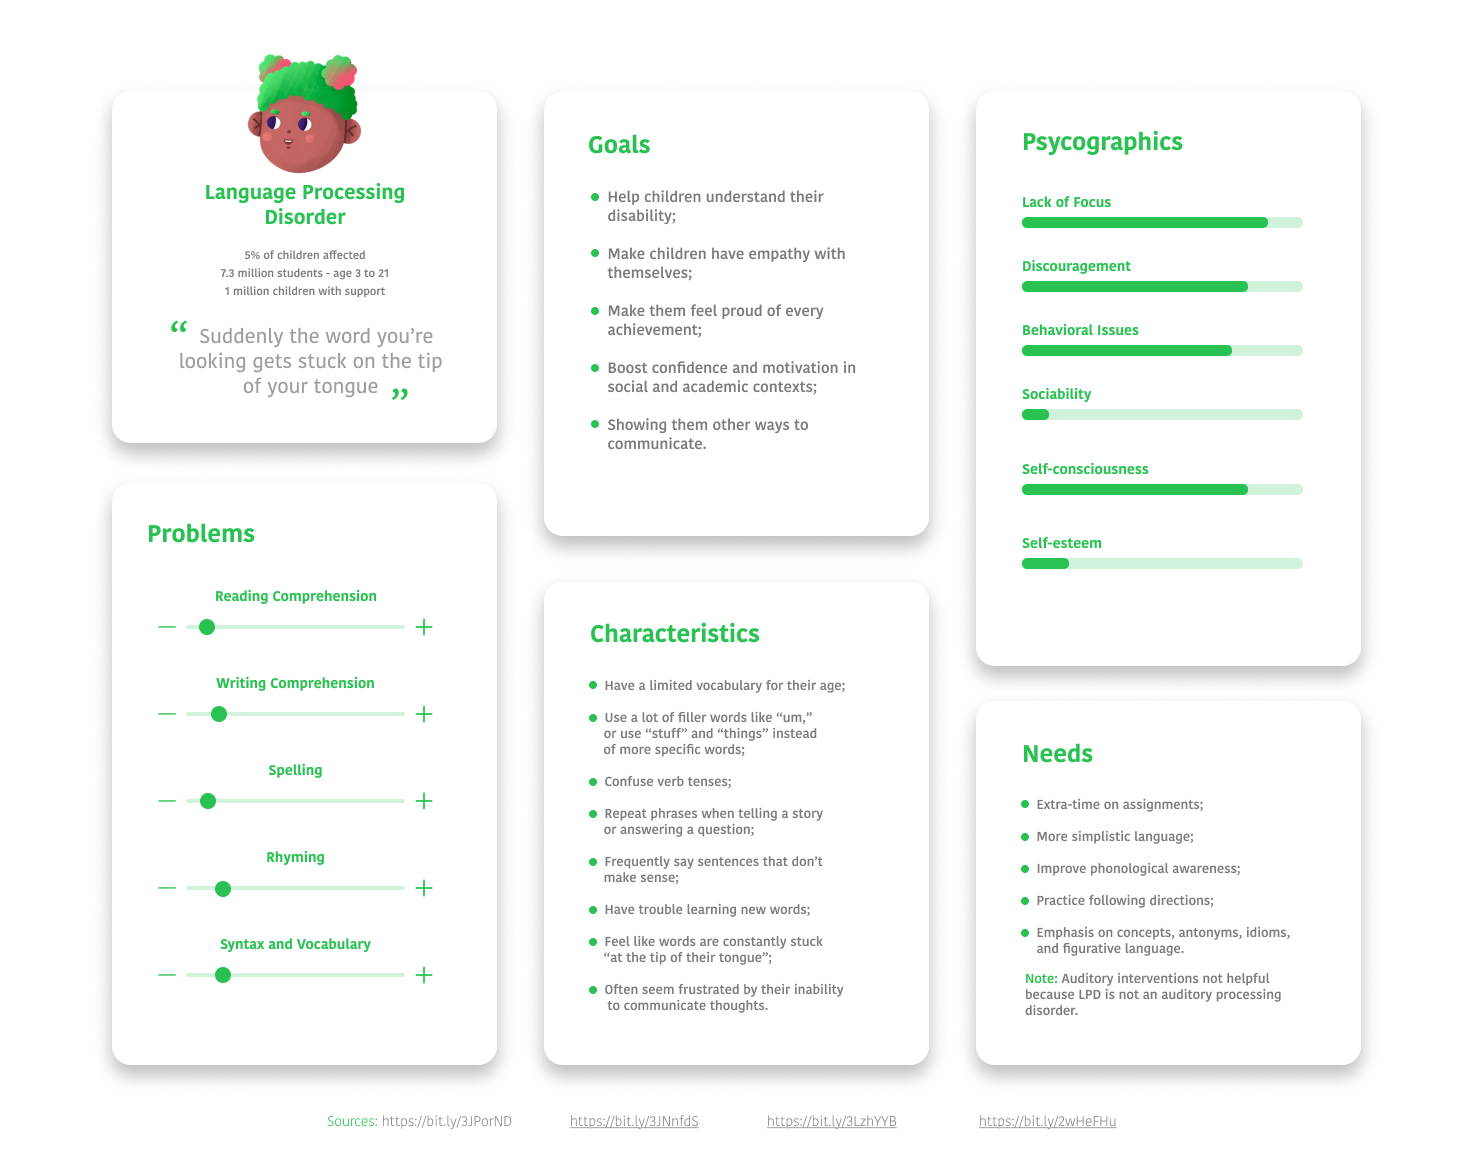
\includegraphics[width=1\linewidth]{Chapters/figma/Language Processing Disorder.png}
    \caption{Language Processing Disorder User Profile}
    \label{fig:lpdUserProfile}
\end{figure}

\paragraph{Goals}
\begin{itemize}
    \item \textbf{Help children understand their disability}: The mini-games aim to provide children with a clear understanding of Language Processing Disorder, its impact on their language skills, and how it does not define their intelligence or potential.
    \item \textbf{Foster empathy and self-acceptance}: By creating an environment that encourages self-compassion and understanding, the mini-games aim to instill a sense of empathy within children towards themselves and others facing similar challenges.
    \item \textbf{Foster pride in achievements}: Recognizing and celebrating every accomplishment, no matter how small, is a key objective of the mini-games.
    \item \textbf{Boost confidence and motivation in social and academic context}: The mini-games aim to enhance children's confidence and motivation to communicate effectively in social and academic settings.
    \item \textbf{Explore alternative communication methods}: The mini-games can introduce children to different ways of communication, such as visual aids, gestures, or assistive technologies, to overcome challenges related with language processing.
\end{itemize}

\paragraph{Psycographics}
\begin{itemize}
    \item \textbf{Low self-esteem}: Struggles with language processing can negatively impact children's self-esteem, making it important to design mini-games that foster a sense of accomplishment and build confidence \cite{vanderbilt}.
    \item \textbf{Low sociability}: Due to communication challenges, children may show a preference for limited social interactions or struggle with initiating and maintaining conversations \cite{greatspeech}.
    \item \textbf{High lack of focus}: Children with LPD may struggle with keeping attention and concentration, making it important to design engaging and interactive mini-games \cite{vanderbilt}.
    \item \textbf{High discouragement}: Difficulties in language processing can lead to frustration and discouragement in academic and social contexts.
    \item \textbf{High behavioral issues}: Children with Language Processing Disorder may exhibit behavioral challenges stemming from their communication difficulties \cite{vanderbilt}.
    \item \textbf{High self-consciousness}: Language difficulties can make children self-conscious about their communication abilities, leading to heightened self-awareness in social and educational settings \cite{additude}.
\end{itemize}

\paragraph{Problems}
\begin{itemize}
    \item \textbf{Reading and Writing Comprehension}: Difficulties in understanding and extracting meaning from written text and expressing thoughts in writing \cite{vanderbilt}.
    \item \textbf{Spelling}: Challenges in accurately spelling words due to difficulties in phonemic awareness and sound-letter correspondence \cite{vanderbilt}.
    \item \textbf{Rhyming}: Difficulty recognizing and generating rhyming words, impacting phonological awareness \cite{vanderbilt}.
    \item \textbf{Syntax and Vocabulary}: Challenges with understanding and using grammatical rules and acquiring and retaining a wide range of vocabulary \cite{additude}.
\end{itemize}

\paragraph{Characteristics}
\begin{itemize}
    \item \textbf{Limited vocabulary for their age}: They may have a smaller repertoire of words compared to their peers \cite{additude}.
    \item \textbf{Use of filler words and vague language}: They may rely on filler words like ''hum'' or use general terms like ''stuff'' and ''things'' instead of specific words \cite{additude}.
    \item \textbf{Confusion with verb tenses}: Difficulties in using and understanding appropriate verb tenses \cite{greatspeech}.
    \item \textbf{Repetition of phrases}: They may repeat phrases when telling stories or answering questions \cite{additude}.
    \item \textbf{Incoherent sentences}: Frequent production of sentences that do not make sense or lack cohesion \cite{additude}.
    \item \textbf{Trouble learning new words}: Challenges in acquiring and retaining new vocabulary \cite{additude}.
    \item \textbf{Tip-of-the-tongue phenomenon}: Feelings of frustration when they cannot retrieve specific words or express their thoughts \cite{additude}.
\end{itemize}

\paragraph{Needs}
\begin{itemize}
    \item \textbf{Extra time on assignments}: Providing additional time for completing tasks and assignments to accommodate the slower processing speed \cite{vanderbilt}.
    \item \textbf{Simplified language}: Using clear and concise language that is appropriate for the children's understanding level and to avoid complex sentence structures \cite{additude}.
    \item \textbf{Improving phonological awareness}: Incorporating activities in the mini-games that focus on recognizing and manipulating sounds within words, such as rhyming, segmenting, and blending \cite{vanderbilt}.
    \item \textbf{Practice following directions}: Designing mini-games that involve following sequential instructions to improve understanding and processing of spoken language \cite{vanderbilt}.
    \item \textbf{Emphasis on concepts, antonyms, idioms, and figurative language}: Including activities that target understanding and using abstract language concepts, such as opposites, idiomatic expressions, and figurative language, to expand their language skills \cite{vanderbilt}.
\end{itemize}

